\documentclass{article}
\usepackage[english]{babel}
\usepackage[letterpaper, margin=1in]{geometry}

\usepackage{amsmath}
\usepackage{graphicx}
\usepackage[colorlinks=true, allcolors=blue]{hyperref}
\usepackage{array,booktabs,ragged2e}

\usepackage[table]{xcolor}
\setlength{\arrayrulewidth}{0.5mm}
\setlength{\tabcolsep}{18pt}

\title{Matador Portfolio Analysis Report}
\author{Understanding Your Portfolio's Performance on a Deeper Level}

\begin{document}

\maketitle

\section*{Summary Statistics}

\begin{table}[h!]
\begin{center}
{\rowcolors{2}{}{gray!20}
\\newcolumntype{R}[1]{>{\RaggedLeft\arraybackslash}p{#1}}
\begin{tabular}{|c|c|}\hline 
 & \textbf{Algo 1}  \\ \hline 
Annual Return & 76.59 \\ \hline
 Cumulative Return & 3598.99 \\ \hline
 Annual Volatility & 24.65 \\ \hline
 Skewness & 0.08 \\ \hline
 Kurtosis & 6.54 \\ \hline
 Sharpe Ratio & 2.69 \\ \hline
 Calmar Ratio & 2.61 \\ \hline
 Stability & 0.99 \\ \hline
 Max Drawdown & -29.32 \\ \hline
 Sortino Ratio & 4.28 \\ \hline
 Tail Ratio & 1.16 \\ \hline
 Daily VaR & -1.97 \\ \hline
 Daily Conditional VaR & -3.03 \\ \hline
 Alpha ($\alpha$) & 0.63 \\ \hline
 Beta ($\beta$) & 0.50 \\ \hline
 \end{tabular}
\caption{Backtest Statistics for trading BAC from 1-4-2016 to 8-11-2022}
}\end{center}
\end{table}


\newpage
 \section*{Cumulative Returns Plot}
\begin{figure}[h!]
    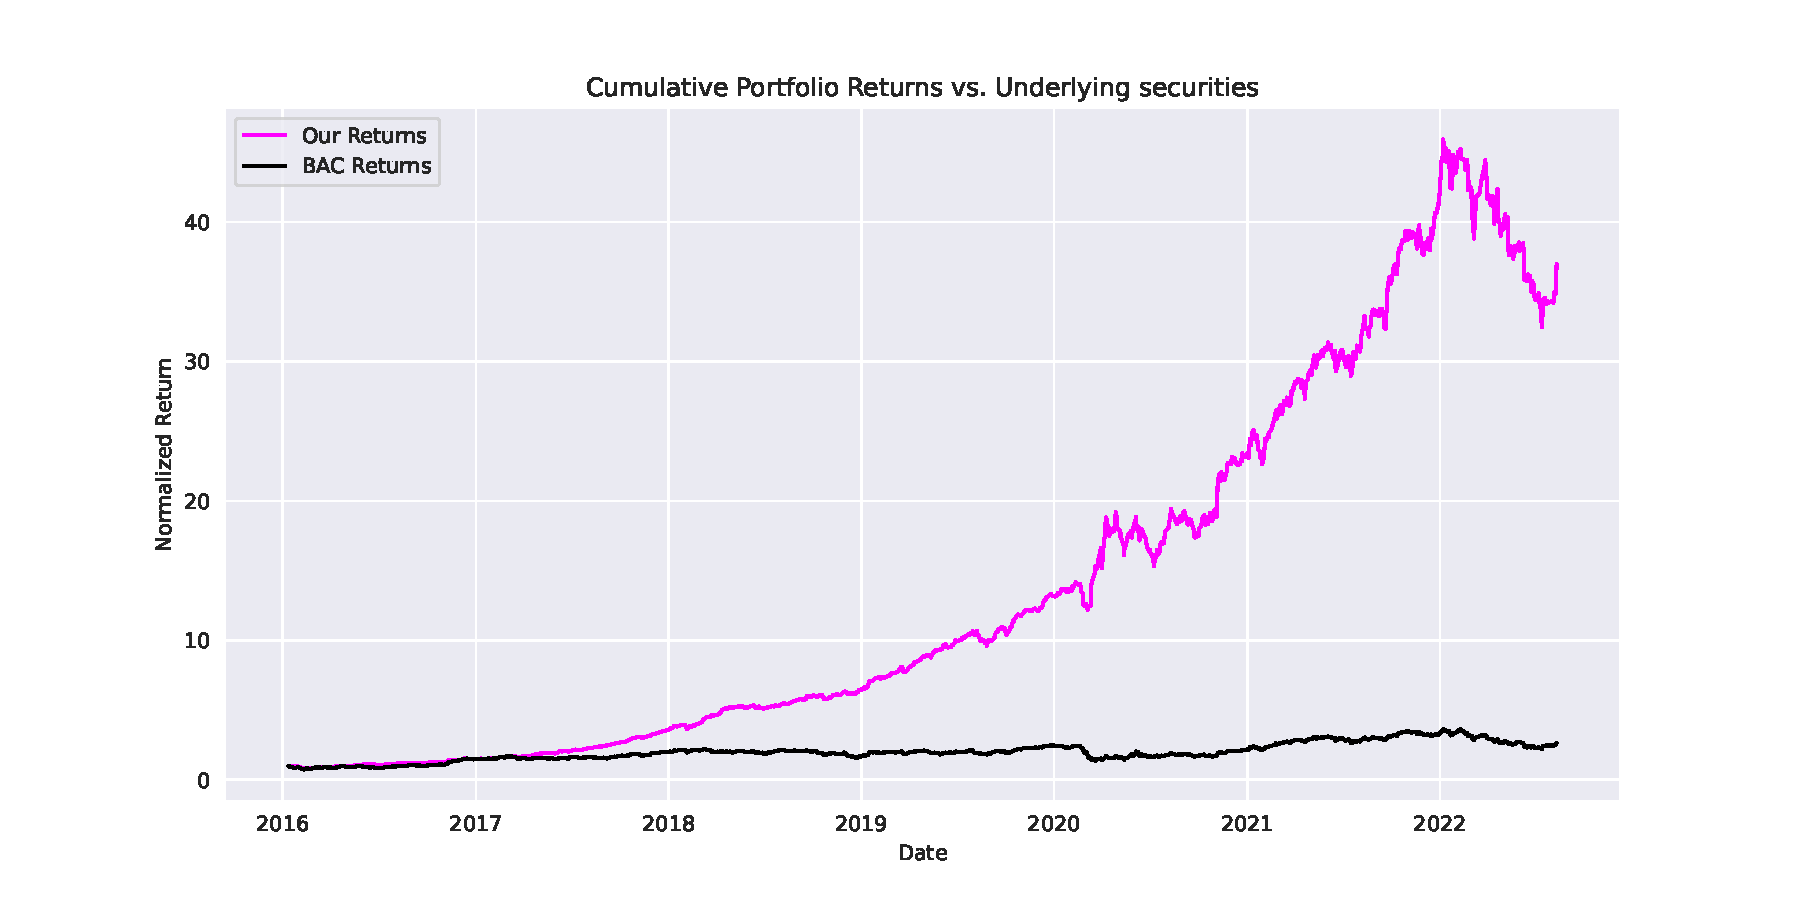
\includegraphics[width=\\textwidth]{cum_ret.pdf}
    \label{fig:my_label}
\end{figure}

\section*{Period Wise Returns Plot}
TODO


\newpage 
\section*{Underwater Plot}
\begin{figure}[h!]
    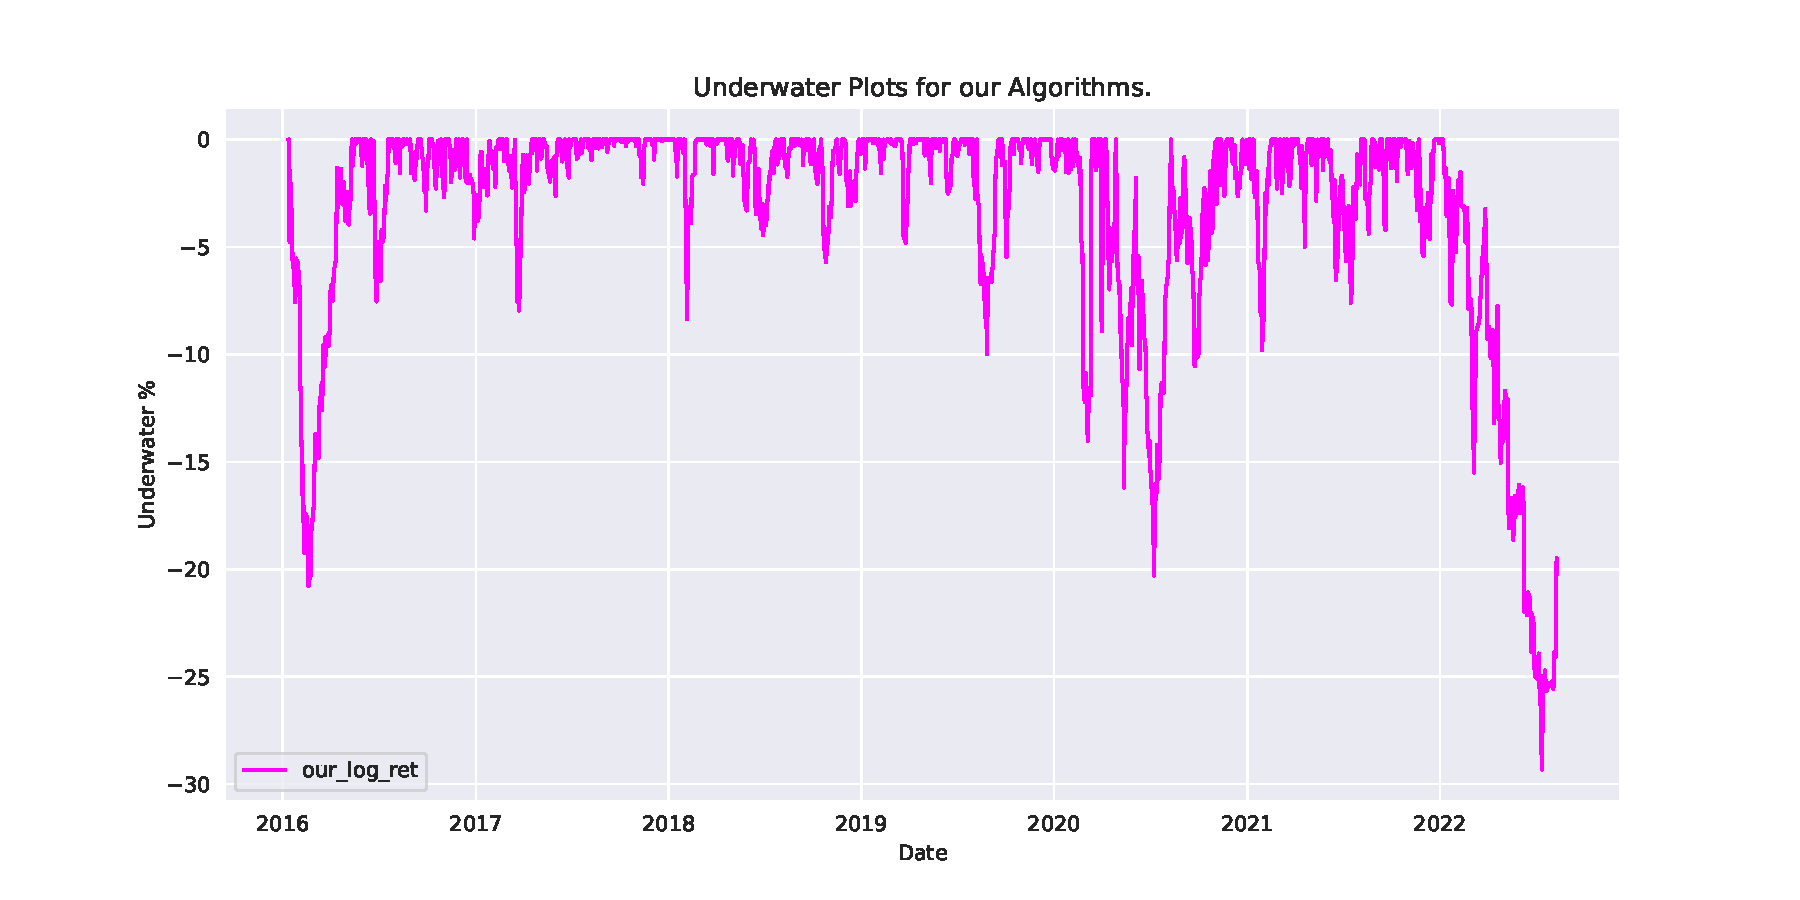
\includegraphics[width=\\textwidth]{underwater.pdf}
    \label{fig:my_label}
\end{figure}

\section*{Other things}

\end{document}
